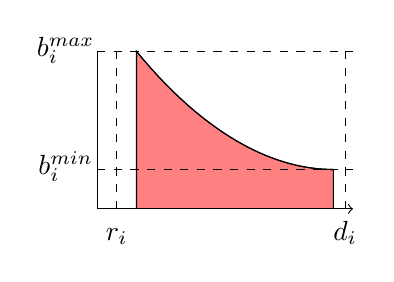
\begin{tikzpicture}
  [scale=0.5]
  \node (O) at (0,0) {};
  \onslide<4->{  
    \path[draw, fill=red!50] (1,0) -- (1,4) parabola [bend at end] (6,1) -- (6,0); 
  }
  \onslide<2->{
    \node[label={[shift={(0,-0.7)}]$r_i$}]  at (0.5,0) {};
    \node[label={[shift={(0,-0.7)}]$d_i$}]  at (6.3,0) {};
    \draw[dashed] (0.5,0) -- (0.5,4);
    \draw[dashed] (6.3,0) -- (6.3,4);
  }
  \onslide<3->{
    \node[label={[shift={(-0.4,-0.4)}]$b_i^{min}$}]  at (0,1) {};
    \node[label={[shift={(-0.4,-0.4)}]$b_i^{max}$}]  at (0,4) {};
    \draw[dashed] (0,1) -- (6.5,1);
    \draw[dashed] (0,4) -- (6.5,4);}
  
  
  \draw (O.center) -- (0,4);
  \draw[->] (O.center) -- (6.5,0);
  
  \draw (1,4) -- (1,0);
  
  
  \path[draw] (1,4) parabola [bend at end] (6,1); 
  
  \draw (6,1) -- (6,0);
\end{tikzpicture}
